%!TEX root = ../index.tex

\newpage
\section{Server} % (fold)
\label{sec:Server}

\subsection{Einleitung} % (fold)
\label{sub:Einleitung}
Um einen OL einfach durch einen neuen zu ersetzen, wird ein zentraler Webserver verwendet. Das sogenannte Backend vereinfacht die Erstellung von OL indem es ermöglicht solche über ein Webformular einzutragen.
% subsection Einleitung (end)

\subsection{Technologie} % (fold)
\label{sub:Technologie}
Da das Backend nicht zentraler Bestandteil dieser Arbeit ist, wurde hier auf schon vorhandene Kenntnisse der Programmiersprache Python und auf Erfahrungen mit dem Django Framework aufgebaut.\\
Django ist ein weit verbreitetes Webframework, welches sich zusammen mit Piston gut für ein solches Projekt eignet.
% subsection Technologie (end)

\subsection{Hosting Evaluation} % (fold)
\label{sub:Hosting Evaluation}
Da Django Applikationen nicht auf jedem Webserver ohne weiteres lauffähig sind, und ein kostenarmer Betrieb auch nach dem Abschliessen dieser Arbeit erzielt werden soll, wurden hier die Bestehenden Applikations Hosting Services ins Auge gefasst.

\subsubsection{Google App Engine} % (fold)
\label{ssub:Google App Engine}
Google betreibt mit der App Engine einen Dienst welche sehr gut Skalierbar ist und für kleine Datenaufkommen auch gratis ist.\\
Jedoch unterstützte die App Engine zu Beginn dieser Arbeit noch keine Relationale Datenbank, was den Programmieraufwand beträchtlich erhöht hätte.
% subsubsection Google App Engnine (end)

\subsubsection{Heroku} % (fold)
\label{ssub:Heroku}
Heroku ist vor allem durch seinen Rails Hosting Service bekannt geworden. Jedoch ist es nun auch möglich diverse andere Frameworks und Sprachen über eigene Scripte einzubinden. Jedoch war dies zu Beginn dieser Arbeit noch nicht so ausgereift und basierte teilweise auf nicht für produktiv Umgebungen konzipierten Anwendungen.
% subsubsection Heroku (end)

\subsubsection{Djangy} % (fold)
\label{ssub:Djangy}
Dieser vielversprechende Service wurde leider kurz vor dieser Arbeit eingestellt, da die Betreiber sich dagegen entschieden haben, Geld aufzunehmen um schneller wachsen zu können.
% subsubsection Djangy (end)

\subsubsection{ep.io} % (fold)
\label{ssub:ep.io}
ep.io ist seit langer Zeit in der Beta Phase und ist nur mit einer persönlichen Einladung nutzbar, jedoch lässt sich ep.io gut mit dem oben aufgeführten Djangy Service Vergleichen. Ein weiterer Vorteil gegenüber App Engine und Heroku ist, dass sich ep.io auf Django Hosting und nicht Web Applikationen im Allgemeinen spezialisiert hat.
% subsubsection ep.io (end)

% subsection Hosting Evaluation (end)

\subsection{Hosting Entscheidung} % (fold)
\label{sub:Hosting Entscheidung}
Da Marc Egli nach über einem halben Jahr Wartezeit noch rechtzeitig als Testbenutzer von ep.io zugelassen wurde und ep.io für unsere Zwecke gratis ist, haben wir uns dafür entschieden ep.io zu auszuprobieren.
% subsection Hosting Entscheidung (end)

\subsection{Bedienung} % (fold)
\label{sub:Bedienung}
Da es sich hier um einen Prototypen handelt wurde das Backend gezielt einfach gehalten. Mittels Passwort kann man sich im System anmelden (Abbildung~\ref{fig:admin-login}) um darin Änderungen vorzunehmen. Danach landet man automatisch in der Übersicht (Abbildung~\ref{fig:admin-index}), von hier aus können diverse Arbeiten erledigt werden. Unter den Menupunkten "`Users"' und "`Groups"' können weitere Benutzer hinzugefügt werden oder bestehenden Benutzern Rechte erteilt und wieder entzogen werden.

\begin{figure}[H]
	\centering			      
        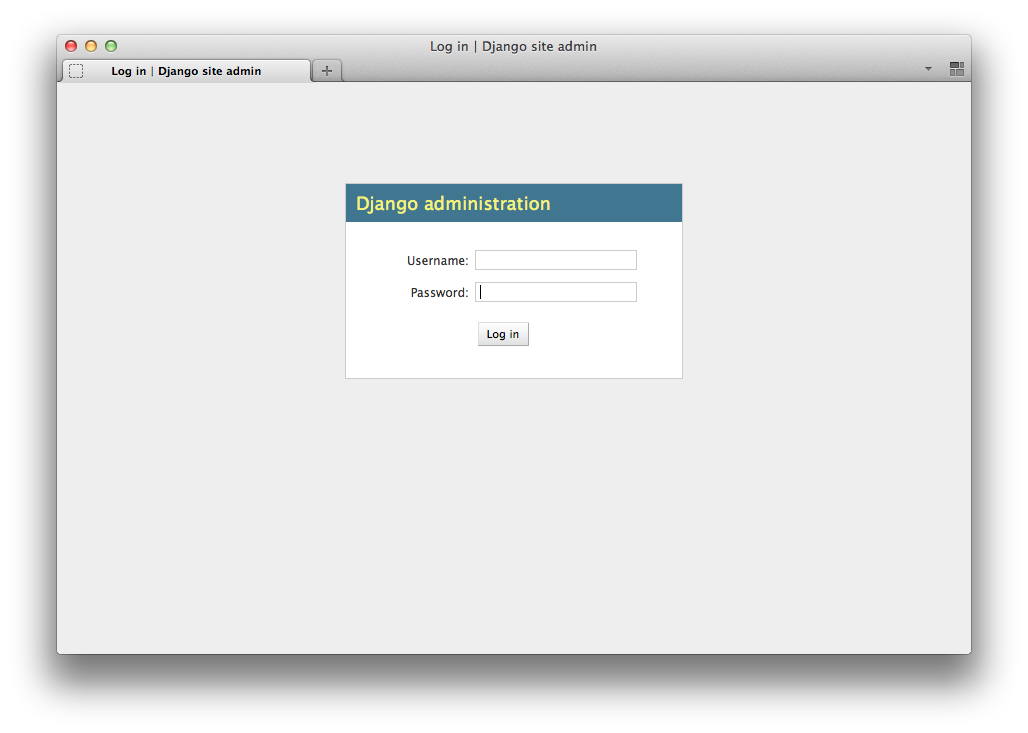
\includegraphics[scale=0.35]{images/admin-login.png}\\
		\caption{Login Screen}
	\label{fig:admin-login}
\end{figure}

\begin{figure}[H]
	\centering			      
        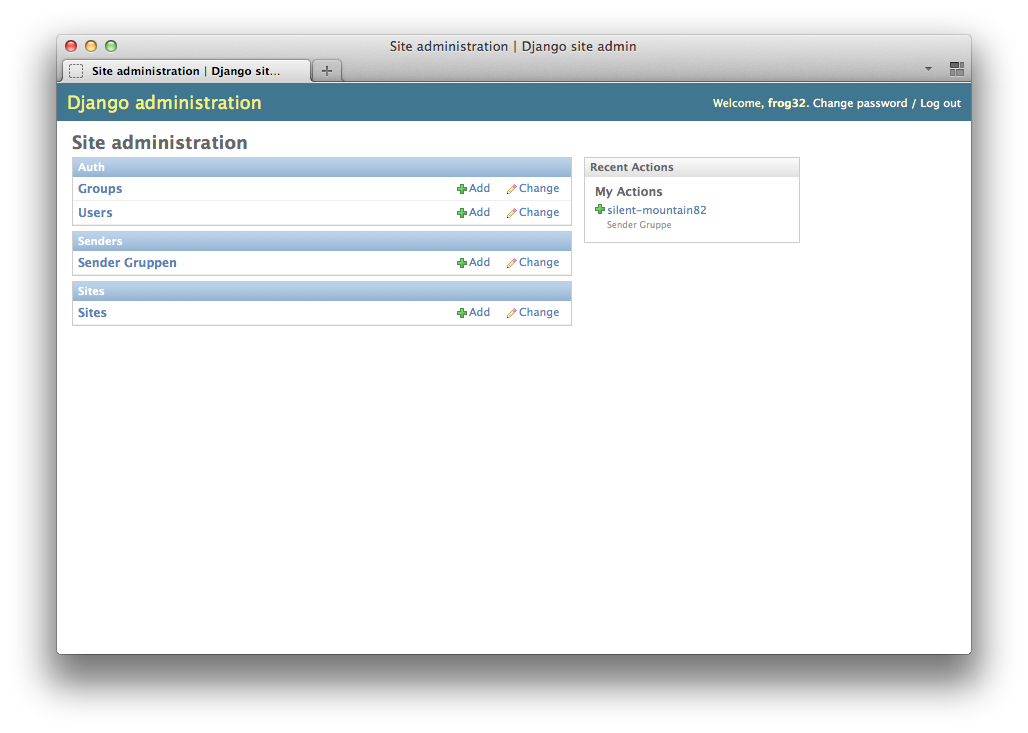
\includegraphics[scale=0.35]{images/admin-index.png}\\
		\caption{Admin Übersicht}
	\label{fig:admin-index}
\end{figure}

Unter dem Menupunkt "`Sender Gruppen"' werden die Fuchsjagd Sender in Gruppen organisiert erfasst. Durch einen Klick auf den Menupunkt gelangt man in die Sendergruppen Übersicht (Abbildung~\ref{fig:group-index}). Hier können bestehende Gruppen durch anklicken geöffnet und editiert werden und über den "`Add Sender Gruppe"' Button können neue Gruppen erfasst werden.

\begin{figure}[H]
	\centering			      
        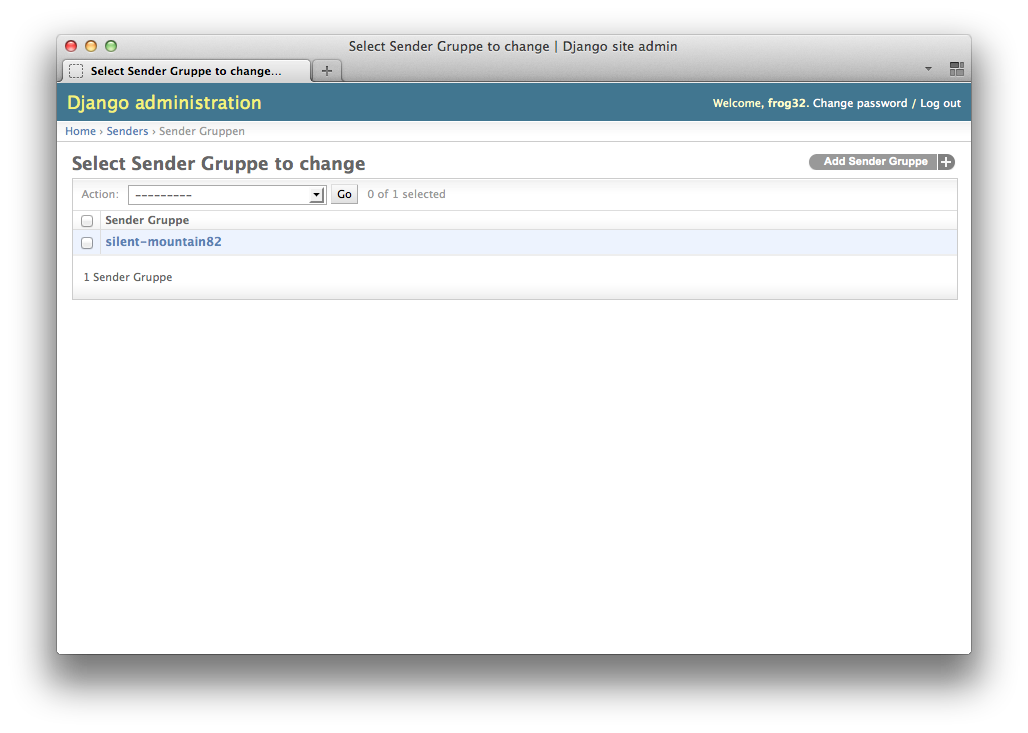
\includegraphics[scale=0.35]{images/group-index.png}\\
		\caption{Listenansicht der einzelnen Sendergruppen}
	\label{fig:group-index}
\end{figure}

\begin{figure}[H]
	\centering			      
        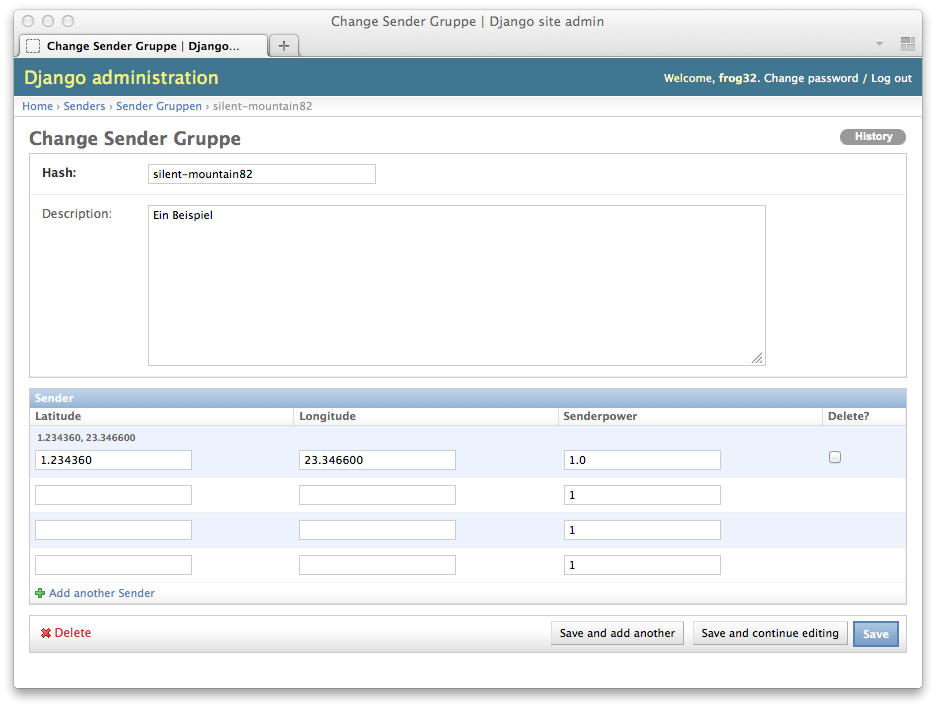
\includegraphics[scale=0.35]{images/group-edit.png}\\
		\caption{Sendergruppe editieren}
	\label{fig:group-edit}
\end{figure}

% subsection Bedienung (end)
% section Server (end)